\documentclass[aspectratio=169]{beamer}
% \documentclass[aspectratio=169,handout]{beamer}

\usetheme[titleformat=regular%
,numbering=fraction% use slide numbers
]{metropolis}
\metroset{%
  progressbar=foot,%
  %background=dark,
  block=fill
}
\only<handout>{\metroset{sectionpage=none}}
\only<handout>{\usecolortheme{dove}}
\usepackage{appendixnumberbeamer} % separate appendix
\usepackage[citestyle=authortitle,sorting=none]{biblatex}
\setbeamerfont{footnote}{size=\tiny}
\addbibresource{mae.bib}

% multimedia in beamer presentations
\usepackage{multimedia}

% adding some better facilities to latex such as proper booleans
\usepackage{etoolbox}

% Unicode math symbols for XeLaTeX
\usepackage{mathrsfs}

% standard math packages
\usepackage{amssymb}
\usepackage{amsthm}
\usepackage{amsmath}
\usepackage{amstext}
\usepackage{mathabx}
\usepackage{stmaryrd}
% math tools for amsmath
\usepackage{mathtools}

\usepackage{proof}

\usepackage{pgfpages}

\usepackage{listings}
\usepackage{xcolor}

% subfigures, subfloats
\usepackage{subcaption}

% for multiinclude
\usepackage{xmpmulti}

% tikz & friends

\usepackage{galois}
\usepackage{tikz}
\usetikzlibrary{fit,calc,shapes,arrows.meta,patterns,backgrounds}
\usetikzlibrary{decorations.pathmorphing}
\usetikzlibrary{cd}
\usepackage[beamer]{hf-tikz}

% for author-title-year citing
\usepackage{xpatch}

\newcommand{\tikzmark}[1]{%
  \tikz[overlay,remember picture,baseline] \node [anchor=base] (#1) {};}

\newenvironment{tightcenter}{%
  \setlength\topsep{0pt}
  \setlength\parskip{0pt}
  \begin{center}
}{%
  \end{center}
}

% new colors
\definecolor{lightblue}{RGB}{217,220,253}
\definecolor{lightred}{RGB}{251,216,218}

\DeclareMathOperator{\pw}{\mathcal{P}} % powerset
\newcommand{\fset}[1]{\mathsf{#1}}
\newcommand{\nats}{\mathbb{N}}
\newcommand{\zahlen}{\mathbb{Z}}
\newcommand{\bools}{\mathbb{B}}
\newcommand{\Set}[1]{\left\{#1\right\}}
\newcommand{\true}{\kw{true}}
\newcommand{\false}{\kw{false}}
\newcommand{\sidenote}[1]{\hfill\quad \textsf{#1}}

\newcommand{\disunion}{+}

% named set
\newcommand{\ns}[1]{\mathit{#1}}
% function
\newcommand{\fn}[1]{\mathrm{#1}}
% "vector of"
\newcommand{\vo}[1]{\overrightarrow{#1}}
% "set of"
\newcommand{\setOf}[1]{\overline{#1}}
% syntactic tag
\newcommand{\sTag}[2]{\textsf{\textbf{#1}}\,#2}
% keyword
\newcommand{\kw}[1]{\texttt{#1}}
% usual suspects
\newcommand{\State}{\ns{State}}
\newcommand{\Value}{\ns{Value}}
\newcommand{\Stmt}{\ns{Stmt}}
\newcommand{\Env}{\ns{Env}}
\newcommand{\Store}{\ns{Store}}
\newcommand{\Kont}{\ns{Kont}}
% syntactic domains
\newcommand{\Exp}{\ns{Exp}}
\newcommand{\Var}{\ns{Var}}
\newcommand{\Addr}{\ns{Addr}}
% put a value to a pointer
\newcommand{\update}{\leftarrow}

% ebnf
\newcommand{\eDEF}{\,::=\;}
\newcommand{\eOR}{\;\vert\;}

\newcommand{\widen}{\nabla}

% \newcommand{\|}{\,\vert\,}

\newcommand{\todo}[1]{\iftoggle{TODO}{\textcolor{red}{TODO: #1}}{}}
% ceiling and floor symbols
\DeclarePairedDelimiter\ceil{\lceil}{\rceil}
\DeclarePairedDelimiter\floor{\lfloor}{\rfloor}

% big O notation
\DeclareMathOperator{\bigO}{O}

% fixed points
\DeclareMathOperator{\lfp}{lfp}

% print both years for bibliography
\renewbibmacro*{cite:labelyear+extrayear}{%
\iffieldundef{labelyear}
{}
{\printtext[bibhyperref]{%
\iffieldundef{origyear}{}{\printfield{origyear}\addslash}%   <--- added
\printfield{labelyear}%
\printfield{extrayear}}}}

\renewbibmacro*{date+extrayear}{%
\iffieldundef{year}
{}
{\printtext[parens]{%
\iffieldundef{origyear}{}{\printfield{origyear}\addslash}%  <--- added
\printdateextra}}}

% overlay an image
\def\Put(#1,#2)#3{\leavevmode\makebox(0,0){\put(#1,#2){#3}}}

% text over symbols nicely, requires amsmath for overset
\newcommand\textoverop[2]{\mathrel{\overset{\makebox[0pt]{\mbox{\normalfont\tiny\sffamily #1}}}{#2}}}

% special arrows
\newcommand\monarrow{\textoverop{mon}{\rightarrow}}

% theorems
\newtheorem{thm}{Theorem}
\newtheorem{eg}{Example}

\newcommand{\abscolor}[1]{\textcolor{mLightBrown}{#1}}
\newcommand{\concolor}[1]{\textcolor{mLightGreen}{#1}}
\newcommand{\abst}[1]{#1^{\#}}

\newcommand{\step}{\rightsquigarrow}

\newcommand{\altm}{\; {\color{black}\mid}\; }

% listings setup
\lstset{basicstyle=\tiny\ttfamily,columns=fixed}

\xapptobibmacro{cite}{\setunit{\nametitledelim}\printfield{year}}{}{}

%%% Local Variables:
%%% mode: latex
%%% TeX-master: "main"
%%% TeX-engine: xetex
%%% End:


\only<handout>{
  \pgfpagesuselayout{4 on 1}[letterpaper,border shrink=5mm,landscape]
}

\newtoggle{notes}
%\only<beamer>{\toggletrue{notes}}

% add notes:
\iftoggle{notes}{
  \makeatletter
  \def\beamer@framenotesbegin{% at beginning of slide
    %\gdef\beamer@noteitems{}%
    %\gdef\beamer@notes{}%
    \usebeamercolor[fg]{normal text}
  }
  \makeatother
  \setbeamertemplate{note page}[plain]
  \setbeamerfont{note page}{size=\footnotesize}
  \setbeameroption{show notes on second screen=right}
}{}

\newtoggle{labdemo}
%\toggletrue{labdemo}
\newtoggle{TODO}
\toggletrue{TODO}

\title[Major Area Exam]{Memory Safety in Systems Languages} %Techniques for
%\subtitle{Tradeoffs in Efficiency and Completeness}
%\subtitle{A Balancing Act}
\subtitle{Major Area Exam}
\date{June 11, 2018}
\author{Michael Christensen}
\institute[UCSB]{
  \normalsize
  {\large \bfseries Committee:}\\
  Ben Hardekopf (\,$\vcenter{\hbox{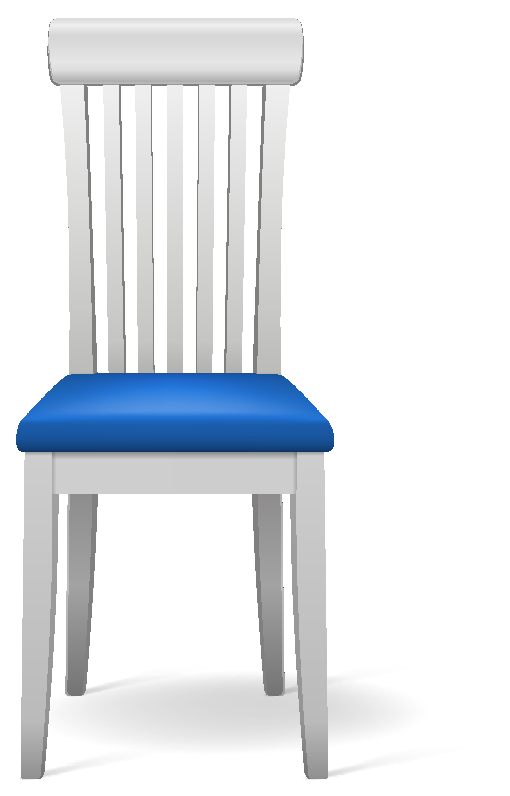
\includegraphics[height=1em]{chair/file.eps}}}$) \quad
  Tim Sherwood \quad
  Rich Wolski
}
\titlegraphic{\hfill
\includegraphics[width=2.25cm]{ucsbseal_cmyk.pdf}}

\begin{document}
\maketitle

\metroset{numbering=none}
\begin{frame}<beamer>[noframenumbering]
  \frametitle{Outline}
  \tableofcontents
\end{frame}
\metroset{numbering=fraction}

\section{Motivation}
\begin{frame}{What is a System?}
Infrastructure software upon which applications are built
% (compilers, garbage collectors, file systems, drivers, etc.)
\\
    \vspace{0.2in}
\pause
Operating Systems
  \begin{itemize}[<+->]
      \item Purpose % i.e. they need to be able to do this
          \begin{itemize}
          \item Process abstraction
          \item Named resource management
              \begin{itemize}
                  \item Multiplex physical hardware resources
                  \item Partition and abstract \textbf{memory}
              \end{itemize}
          \end{itemize}
      \item Goals: low overhead, robustness, security
  \end{itemize}
\end{frame}

%\notes{
% isolation third item for os
% files: hide peculiarites of disks/I/O decives, abstract model of device-indepdent files
% address space: virtual memory + protection
% process: running program container (registers, files, alarms, address space, etc.)
%}

\begin{frame}{Systems Languages}
\begin{itemize}[<+->]
    \item Past systems languages: \tiny{ALGOL, PL/I, Fortran, BCPL/B, C, Mesa/Cedar, Pascal/Modula-2/Oberon, C++, ...}
    \item C: the de-facto standard
        \begin{itemize}
            \item Data structure representation control
            \item Memory management control % don't need to use stdlib either
            \item Complete mutability via pointers % define what I mean here
            \item Performant
        \end{itemize}
    \item C: the unsafe standard
        \begin{itemize}
            \item Unchecked array operations $\Rightarrow$ buffer overflows
            \item Pointers $\equiv$ arrays $\Rightarrow$ hazardous pointer arithmetic
            \item Unsafe casts $\Rightarrow$ read/write arbitrary addresses
            \item Aliasing $\Rightarrow$ dangling pointers, double frees, null dereferences
        \end{itemize}
\end{itemize}
\end{frame}

%\notes{
% possibly add OS lang was used for, date
% ALGOL: formally defined syntax
% Mesa, Cedar: rich exceptions, GC
% Pascal (1971), Modula-2 (1982), Oberon (1988) % structured programming, records, pointers, dynamic allocation, information hiding, objects
% see mae3.org, mae4.org
%}

\begin{frame}{Memory Safety}
\begin{itemize}[<+->]
    \item Memory safety error: ``Any dereference of a pointer or subscripted array reference which reads or writes storage outside of the referent'' \footcite{austin_efficient_1994}
        \begin{itemize}
            \item Spatial: outside referent's \alert{address bounds}
            \item Temporal: outside referent's \alert{lifetime}
        \end{itemize}
    \item Ideal technique is
        \begin{itemize}
            \item Efficient and expressive % (hallmarks of C)
            \item Purely static % (no runtime overhead)
            \item Precise % (not overly conservative)
            \item Automatic % (legacy code $\Rightarrow$ no source or memory layout change)
        \end{itemize}
%    \item Non-goals: secrecy, security, concurrency, type safety % but are natural consequences of safety
    \item Memory errors become \alert{type errors}, management happens at \alert{compile-time}
\end{itemize}
\end{frame}

%\notes{
% some of those goals from nagakatte 201*
% undecidability of checking certain dynamic errors
% hard to verify/prove invariants about b/c
  % casts + pointers make c essentially untyped (rondon: type system is only to help know size of bytes to read/write)
  % aliasing
% make bad hard, useful easy
%}

\AtBeginSection[]
{
  \metroset{numbering=none}
  \begin{frame}<beamer>[noframenumbering]
    \frametitle{Outline}
    \tableofcontents[currentsection]
  \end{frame}
  \metroset{numbering=fraction}
}

\only<handout>{
  \addtocounter{framenumber}{1}
}

\section{Spatial Safety}

\begin{frame}[fragile]{Definition and Example}
  \footnotesize
  \begin{columns}[T]
    \begin{column}{0.45\textwidth}
        Foo bar baz
    \end{column}
    \begin{column}{0.45\textwidth}
%      \lstinputlisting[language=C,mathescape]{lst/spatial_plain.c}
       \begin{lstlisting}[language=C,numbers=left,mathescape,basicstyle={\footnotesize\ttfamily}]
int main() {
    printf("hello, world!\n");
}
$$
        \end{lstlisting}
    \end{column}
  \end{columns}
\end{frame}

\subsection{Some Dynamic Approaches}

\begin{frame}[fragile]{Fat Pointers}
  \footnotesize
  \begin{columns}[T]
    \begin{column}{0.45\textwidth}
        Foo bar baz
    \end{column}
    \begin{column}{0.45\textwidth}
%      \lstinputlisting[language=C,mathescape]{lst/spatial_fat.c}
       \begin{lstlisting}[language=C,numbers=left,mathescape,basicstyle={\footnotesize\ttfamily}]
int main() {
    printf("hello, world!\n");
}
$$
        \end{lstlisting}
    \end{column}
  \end{columns}
\end{frame}

\begin{frame}[fragile]{Separate Metadata}
  \footnotesize
  \begin{columns}[T]
    \begin{column}{0.45\textwidth}
        Foo bar baz
    \end{column}
    \begin{column}{0.45\textwidth}
%      \lstinputlisting[language=C,mathescape]{lst/spatial_table.c}
       \begin{lstlisting}[language=C,numbers=left,mathescape,basicstyle={\footnotesize\ttfamily}]
int main() {
    printf("hello, world!\n");
}
$$
        \end{lstlisting}
    \end{column}
  \end{columns}
\end{frame}

\begin{frame}[fragile]{Objects}
  \footnotesize
  \begin{columns}[T]
    \begin{column}{0.45\textwidth}
        Foo bar baz
    \end{column}
    \begin{column}{0.45\textwidth}
%      \lstinputlisting[language=C,mathescape]{lst/spatial_objs.c}
       \begin{lstlisting}[language=C,numbers=left,mathescape,basicstyle={\footnotesize\ttfamily}]
int main() {
    printf("hello, world!\n");
}
$$
        \end{lstlisting}
    \end{column}
  \end{columns}
\end{frame}

\subsection{Some Static Approaches}

\begin{frame}[fragile]{Extended Type Checking}
  \footnotesize
  \begin{columns}[T]
    \begin{column}{0.45\textwidth}
        Foo bar baz
    \end{column}
    \begin{column}{0.45\textwidth}
%      \lstinputlisting[language=C,mathescape]{lst/spatial_etc.c}
       \begin{lstlisting}[language=C,numbers=left,mathescape,basicstyle={\footnotesize\ttfamily}]
int main() {
    printf("hello, world!\n");
}
$$
        \end{lstlisting}
    \end{column}
  \end{columns}
\end{frame}

\begin{frame}[fragile]{LCLint}
  \footnotesize
  \begin{columns}[T]
    \begin{column}{0.45\textwidth}
        Foo bar baz
    \end{column}
    \begin{column}{0.45\textwidth}
%      \lstinputlisting[language=C,mathescape]{lst/spatial_lclint.c}
       \begin{lstlisting}[language=C,numbers=left,mathescape,basicstyle={\footnotesize\ttfamily}]
int main() {
    printf("hello, world!\n");
}
$$
        \end{lstlisting}
    \end{column}
  \end{columns}
\end{frame}

\begin{frame}[fragile]{CSSV}
  \footnotesize
  \begin{columns}[T]
    \begin{column}{0.45\textwidth}
        Foo bar baz
    \end{column}
    \begin{column}{0.45\textwidth}
%      \lstinputlisting[language=C,mathescape]{lst/spatial_cssv.c}
       \begin{lstlisting}[language=C,numbers=left,mathescape,basicstyle={\footnotesize\ttfamily}]
int main() {
    printf("hello, world!\n");
}
$$
        \end{lstlisting}
    \end{column}
  \end{columns}
\end{frame}

% TODO need to introduce type systems, semantics, syntax

\subsection{Dependent Types}

\begin{frame}{foo}
\end{frame}

\section{Temporal Safety}

\begin{frame}[fragile]{Definition and Example}
    \footnotesize
\end{frame}

\end{document}

%%% Local Variables:
%%% mode: latex
%%% TeX-master: t
%%% TeX-engine: xetex
%%% End:
